\chapter{Methods}

\section{Data}
While examining both proposed methods for their suitability for near-infrared colorization, multiple datasets
and two data sources \textit{Caltech Camera Traps} \cite{caltech} and \textit{Snapshot Serengeti} \cite{serengeti} were used.

\subsection{Caltech Camera Traps}
\textit{Caltech Camera Traps} (CCT) is a dataset consisting of $243.100$ images from $140$ camera locations
in the southwestern United States with $21$ animal label categories \cite{caltech}.
In particular, it primarily contains near-infrared images for the night and regular RGB images for images captured during the day.
Approximately $70 \%$ of the overall image set is labeled empty.
Annotations are provided in the \textit{COCO Camera Traps} format, describing meta information via JSON \cite{caltech}
This allows an automatic parsing of the available images as well as efficient access to information about
the images, which comes in useful when creating sub-datasets for training networks.

\subsection{Snapshot Serengeti}
In contrast to the CCT dataset, \textit{Snapshot Serengeti} is a much larger dataset and comes from the Snapshot Serengeti National Park in Tanzania.
It consists of $7.1$ million images through seven seasons of the Snapshot Serengeti Project \cite{serengeti}.
There are $61$ labeled species, where approximately $76\%$ of the images are labeled empty.
Similar to the CCT dataset, Snapshot Serengeti contains near-infrared images as well as RGB images and
is annotated in the COCO Camera Traps format \cite{serengeti}. Therefore, dataset tooling can be used for both datasets.
Unlike the CCT dataset, Snapshot Serengeti employed multiple cameras for images captured at night.
Scoutgard's SG565 cameras produce RGB \textbf{night} images using an \textit{incandescent} flash and DLC Covert II cameras use an infrared flash and therefore produce NIR night images \cite{serengeti}.

\subsection{Subset Generation}
Since both datasets (CCT and Snapshot Serengeti) are substantially larger than processable for training, choosing a subset of these images is essential.
The requirements for this subset strongly influence the training performance of the translation models.

\begin{enumerate}
      \item Both network architectures require the dataset to be divided into an input domain (NIR) and an output domain (RGB). \label{item:requirement-split}
      \item To gain model performance in the main objective, which is to colorize the NIR images of \textit{animals}, it is important to choose only images that contain animals. \label{item:requirement-animal-filter}
      \item Training with a variety of image locations proves to decrease overfitting for the translation, and therefore a uniform distribution of the available locations should be approximated.
            Additionally, utilizing a random crop for each image can also help mitigate overfitting, and therefore, it is suggested. \label{item:requirement-weighted-sampling}
      \item Since most NIR images are taken at night, the network should not be influenced to solve the more difficult
            task of translating images from NIR night to RGB day. This can be achieved by only allowing night images for both
            domains. \label{item:requirement-night}
\end{enumerate}


The \ref{item:requirement-animal-filter}., \ref{item:requirement-weighted-sampling}. and \ref{item:requirement-night}. requirements are all achievable by using the information provided in the COCO format, and therefore,
are already obtainable before downloading a single image.
Only choosing images with animals (\ref{item:requirement-animal-filter}.) is done by a simple filter on the data source before sampling.
The approximately uniform distribution of locations (\ref{item:requirement-weighted-sampling}.) can be archived using a weighted sampling with the inverse of location occurrences as weight.
Filtering for only night images (\ref{item:requirement-night}.) can also be achieved only using metadata:
The COCO format documents the time of recording. Using time zones and geolocations, individual time frames for each day of the year can serve as filters for night images.

Since the COCO format does not provide information about which item is a NIR- and which item is an RGB image (\ref{item:requirement-split}.) \cite{caltech}, that information is not available before downloading.
Because both data sources provide their NIR images with \textit{colored} logos, they are stored in an RGB image where the actual image section has equal values over all three channels.
Therefore, a pragmatic solution is to download the images and compare the three channels in a cropped version of the image (without the logo section).

This whole process can be automated in the form of a mix between a rejection- and an importance sampler:
It samples from the filtered data source with weights by location, downloads the image and rejects a sample if the desired amount of NIR- or RGB images is reached.
Finally, the produced subset can be stored in a compact format to achieve reproducibility across systems and reduce computational time.

\section{CycleGAN}

\subsection{Generative Adversarial Networks}

For image translation, a mapping function $G: \mathcal{X} \to \mathcal{Y}$ shall be learned.
In our case, $\mathcal{X}$ is the input domain of the near-infrared images, whereas $\mathcal{Y}$ is the output domain of the colored RGB images.
For the training, two sets $X = \{\x \in \mathcal{X}\}$, $Y = \{\y \in \mathcal{Y}\}$ are given.
For the unpaired image translation, the mapping function must be learned without any existing $\x \in X$ for which $G(\x)=\y$ is known.
Therefore, supervised learning techniques are not applicable, and unsupervised learning methods must be considered.

\textit{Generative Adversarial Networks} (GANs) provide a way of learning this function by declaring the objective that, for a $\x \in \mathcal{X}$, $G(\x) = \hat{\y}$
should be indistinguishable from images from $\y \in \mathcal{Y}$. GANs achieve this by splitting the training architecture into two networks:
The \textit{generator} $G: \mathcal{X} \to \mathcal{Y}$ that learns the relationship between the two domains and the \textit{discriminator} $D: \mathcal{Y} \to \mathbb{R}$ that learns to
classify possible images from $\mathcal{Y}$ as "real" or "generated".
Both networks optimize each other and play a min-max game:
The generator tries to fool the discriminator into classifying the generated image as "real" and thereby learns to produce \textit{indistinguishable} images from $Y$.
Additionally, the discriminator tries to detect generated images, while also learning the features of the domain $\mathcal{Y}$ by classifying those as "real".

Although this method has already proven to perform well for image translation, it has issues preserving the content.
GANs in general are not restricted in training to map the actual \textbf{content} from the given image
$\x \in X$ to the image produced $G(\x) \in Y$.
For example, one could imagine that the mapping function which maps all $\x$ to some real $\y \in Y$ ($G(\x) = \y$) should perform exceptionally well in terms of its training loss, since the produced image should always be classified as "real".
This case is called \textit{mode collapse} and can be weakened by adding additional structure to the training.

In the following, we will concentrate on two options:
1. Using a \textit{cycle consistency loss} which was introduced by Zhu \textit{et al.} for the network \textit{CycleGAN} \cite{cyclegan_orig}
and 2. using a \textit{contrastive loss} that Park \textit{et al.} introduced into this environment for the network \textit{CUT} \cite{cut}.


\subsection{Cycle-Consistency Loss}

CycleGAN is a network architecture presented by Zhu \textit{et al.} and introduces a \textit{cycle consistency loss} for image translations using GANs.
The idea is that the translation between the two domains should be "cycle consistent", meaning that when translating an image from NIR to RGB and back
to NIR, both NIR images should be approximately equal.
Mathematically, this means that we have an additional function $F: \mathcal{Y} \to \mathcal{X}$ which is approximately the inverse of $G$. For a $\x \in \mathcal{X}$, $F(G(\x)) \approx \x$.
This is encouraged using a \textit{cycle consistency loss} \cite{cyclegan_orig}. We assume that if a $\x$ is recoverable from a $\y = G(\x)$ using $F$, the content of $\x$
is preserved in $\y$ \cite{cyclegan_orig} (\autoref{fig:cycle-gan}).

\begin{figure}[h]
   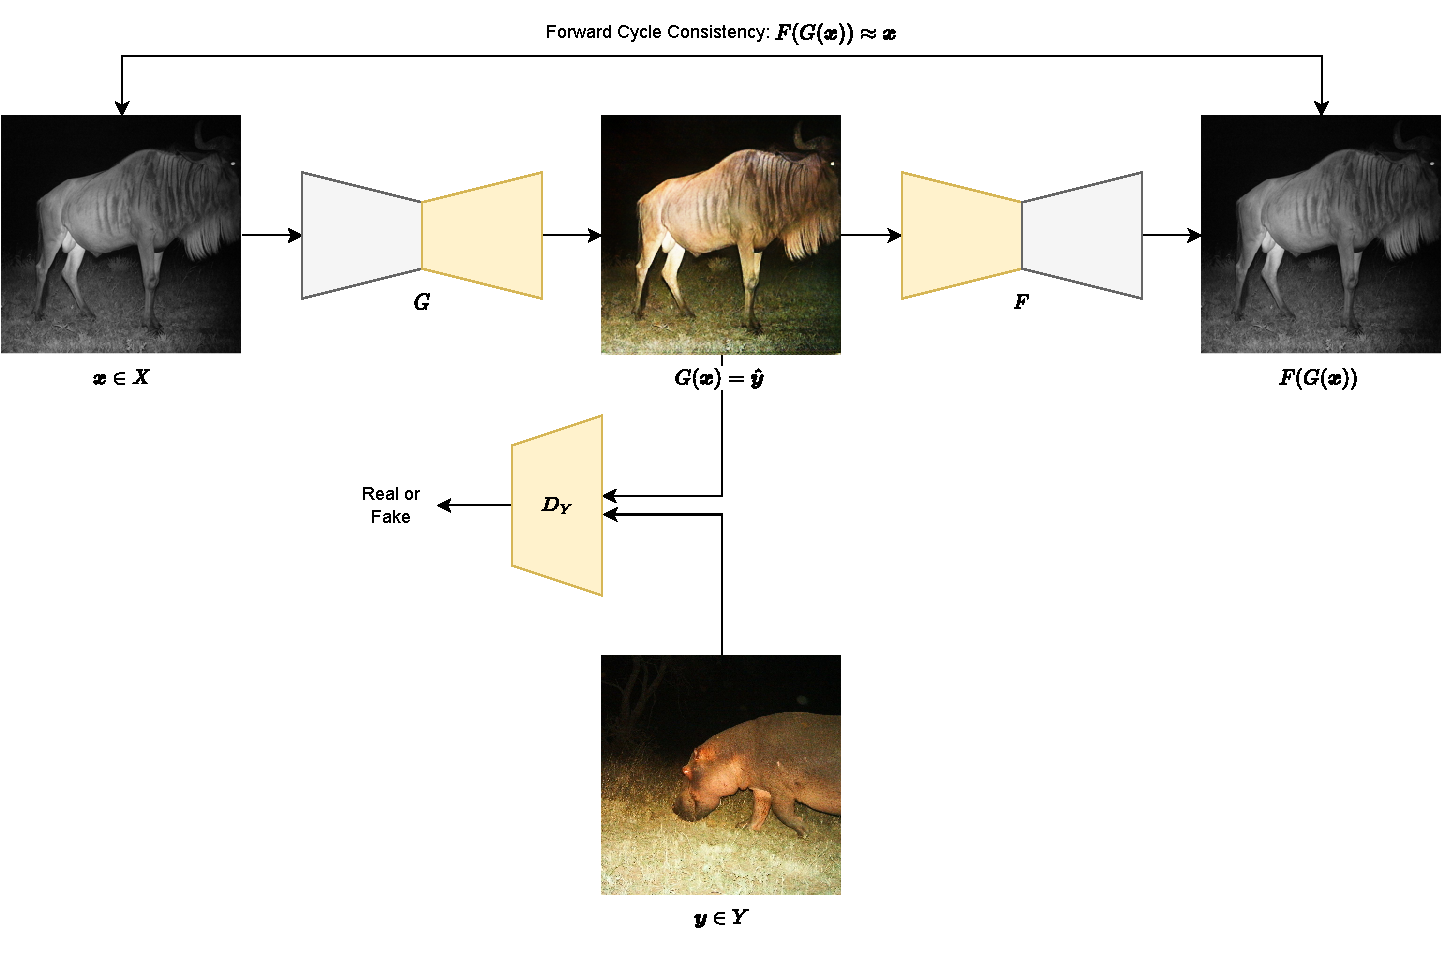
\includegraphics[width=\textwidth]{gfx/CycleGAN.pdf}
   \caption{
      \textbf{CycleGAN Schema.} Two generators $G$ and $F$ translate between both domains. Forward Cycle Consistency is ensured using the input and recovered NIR image.
      The discriminator $D_Y$ encourages the generator $G$ to learn the features of domain $\mathcal{Y}$ \cite{cyclegan_orig,mehri2019colorizing}.
   }
   \label{fig:cycle-gan}
\end{figure}

\subsubsection*{Cycle Consistency Loss}
This objective is written as a loss function $\mathcal{L}_{cyc}(G, F)$ which uses an L1 norm to encourage cycle consistency (\autoref{eqn:cyc}).
In addition to \textit{forward cycle consistency}, CycleGAN also utilizes \textit{backward cycle consistency} which means that for $\y \in \mathcal{Y}$, $G(F(\y)) \approx \y$ \cite{cyclegan_orig} applies, too (\autoref{fig:cycle-gan}).

\begin{equation}
   \label{eqn:cyc}
   \begin{aligned}
      \mathcal{L}_{cyc}(G, F) = \underbrace{\mathbb{E}_{\x \sim X}\left[||F(G(\x)) - \x||_1\right]}_{\text{forward cycle consistency}} +
      \underbrace{\mathbb{E}_{\y \sim Y}\left[||G(F(\y))) - \y||_1\right]}_{\textit{backward cycle consistency}}
   \end{aligned}
\end{equation}

In addition to the L1 cycle consistency loss, Mehri \textit{et al.} propose using \textit{structural similarity index measurement} (SSIM) as the second cycle consistency loss \cite{mehri2019colorizing}.
Contrary to the L1 loss, SSIM measures the differences between the images not by the absolute image intensity values but by comparing two images based on luminance-, contrast- and structural similarity \cite{ssim}.

Using measurements for luminance $l(\y_1, \y_2)$, contrast $c(\y_1,\y_2)$ and structure comparison $s(\y_1, \y_2)$, we can obtain the overall structural similarity
index $SSIM(\y_1, \y_2)$ as multiplication of each component (\autoref{eqn:ssim}) \cite{ssim}.

\begin{equation}
   \label{eqn:ssim}
   \begin{aligned}
      SSIM(\y_1, \y_2) = l(\y_1, \y_2) \cdot c(\y_1,\y_2) \cdot s(\y_1, \y_2)
   \end{aligned}
\end{equation}

The SSIM is obtained using a moving Gaussian window on the image, and therefore the SSIM \textbf{difference} between two images $\overline{SSIM(\y_1,\y_2)}$ is calculated as follows (\autoref{eqn:ssim_difference}).
Let $\y_{1,j}$ and $\y_{2,j}$ be the image contents of the $j$-th local patch using the Gaussian window, where $M$ is the number of Gaussian windows.

\begin{equation}
   \label{eqn:ssim_difference}
   \begin{aligned}
      \overline{SSIM(\y_1,\y_2)} = \frac{1}{M}\sum_{j=1}^{M}1 - SSIM(\y_{1,j},\y_{2,j})
   \end{aligned}
\end{equation}

Finally, the loss of cycle consistency $\mathcal{L}_{SSIM}(G, F)$ can be constructed using the differences in the SSIMs between the images (\autoref{eqn:ssim_loss}).

\begin{equation}
   \label{eqn:ssim_loss}
   \begin{aligned}
      \mathcal{L}_{SSIM}(G,F) & = \mathbb{E}_{\x \sim X}\left[\overline{SSIM(F(G(\x)), \x)}\right] + \mathbb{E}_{\y \sim Y}\left[\overline{SSIM(G(F(\y)), \y)}\right]
   \end{aligned}
\end{equation}


\subsubsection*{Relativistic Adversarial Loss}
For both generators, adversarial discriminators $D_X$ and $D_Y$ are introduced where $D_X$ has the aim of distinguishing between real images
$X$ and generated images $\{F(\y)\}$ and $D_Y$ for $Y$ and $\{G(\x)\}$.
For both, we apply a relativistic GAN, in particular, \textit{RaLSGAN} \cite{mehri2019colorizing,rel_gan}.
\autoref{eqn:ralsgan} demonstrates the RaLSGAN loss for the generator $G$ ($\mathcal{L}^G_{RaLSGAN}(G,D_Y,X,Y)$) and its discriminator
$D_Y$ ($\mathcal{L}^D_{RaLSGAN}(G,D_Y,X,Y)$) (\autoref{fig:cycle-gan}). The loss for $F$ and $D_X$ is defined in the same way as for $G$ and $D_Y$ \cite{rel_gan}.

\begin{equation}
   \label{eqn:ralsgan}
   \begin{aligned}
      \mathcal{L}^{D_Y}_{RaLSGAN}(G,D_Y,X,Y) & = \mathbb{E}_{\y \sim Y}\left[(D_Y(\y) - \mathbb{E}_{\x \sim X} D_Y(G(\x)) - 1)^2 \right] \\
                                             & + \mathbb{E}_{\x \sim X}\left[(D_Y(G(\x)) - \mathbb{E}_{\y \sim Y} D_Y(\y) + 1)^2 \right] \\
      \mathcal{L}^G_{RaLSGAN}(G,D_Y,X,Y)     & = \mathbb{E}_{\x \sim X}\left[(D_Y(G(\x)) - \mathbb{E}_{\y \sim Y} D_Y(\y) - 1)^2 \right] \\
                                             & + \mathbb{E}_{\y \sim Y}\left[(D_Y(\y) - \mathbb{E}_{\x \sim X} D_Y(G(\x)) + 1)^2 \right]
   \end{aligned}
\end{equation}

\subsection*{Identity Loss}
Lastly, the identity loss has the aim of regulating the generator:
If an image already appears like a colored RGB image, it should not be modified.
This leads to the identity loss $\mathcal{L}_{identiy}$ (\autoref{eqn:identity_loss}) \cite{mehri2019colorizing}.

\begin{equation}
   \label{eqn:identity_loss}
   \begin{aligned}
      \mathcal{L}_{identiy}(G, F) = \mathbb{E}_{\x \sim X} \left[||G(\x) - \x||_1\right] + \mathbb{E}_{\y \sim Y} \left[||G(\y) - \y||_1\right]
   \end{aligned}
\end{equation}

\subsection*{Full Objective}
All those four loss functions lead to an additive final loss function (\autoref{eqn:cycle_gan_total_loss}) \cite{mehri2019colorizing}.
$\lambda$ and $\gamma$ are weights for the relative importance of the L1 cycle consistency loss and the identity loss.

\begin{equation}
   \label{eqn:cycle_gan_total_loss}
   \begin{aligned}
      \mathcal{L} = \lambda \mathcal{L}_{cyc} + \mathcal{L}_{SSIM} + \gamma \mathcal{L}_{identity}(G,F) + \mathcal{L}_{RaLSGAN}^G(G,D_Y,X,Y) + \mathcal{L}_{RaLSGAN}^F(F,D_X,Y,X)
   \end{aligned}
\end{equation}

\subsubsection*{U-Net}
In praxis, both functions $G$ and $F$ are generation networks. Contrary to the ResNet generators \cite{resnet} Zhu \textit{et al.} used in the original CycleGAN \cite{cyclegan_orig},
Mehri \textit{et al.} propose U-Net generators \cite{unet}, because they perform better in learning the color \cite{mehri2019colorizing}.
Additionally, U-Net generators also need less computational time for training compared to ResNet \cite{mehri2019colorizing}.
We input all three (equal) channels of the NIR image into the generator and receive an RGB image as output.
All activations of the encode-blocks (except the last one) are inputs for two blocks:
The following encode- as well as the corresponding decode-block. This is called a skip connection \cite{unet} (\autoref{fig:unet}). All decode-blocks (except the first one) receive input from the previous decode-block, as well as the corresponding encode-block.
This leads to an architecture that can learn to "choose" how deep the feature abstraction should be \cite{unet}.

\begin{figure}[h]
   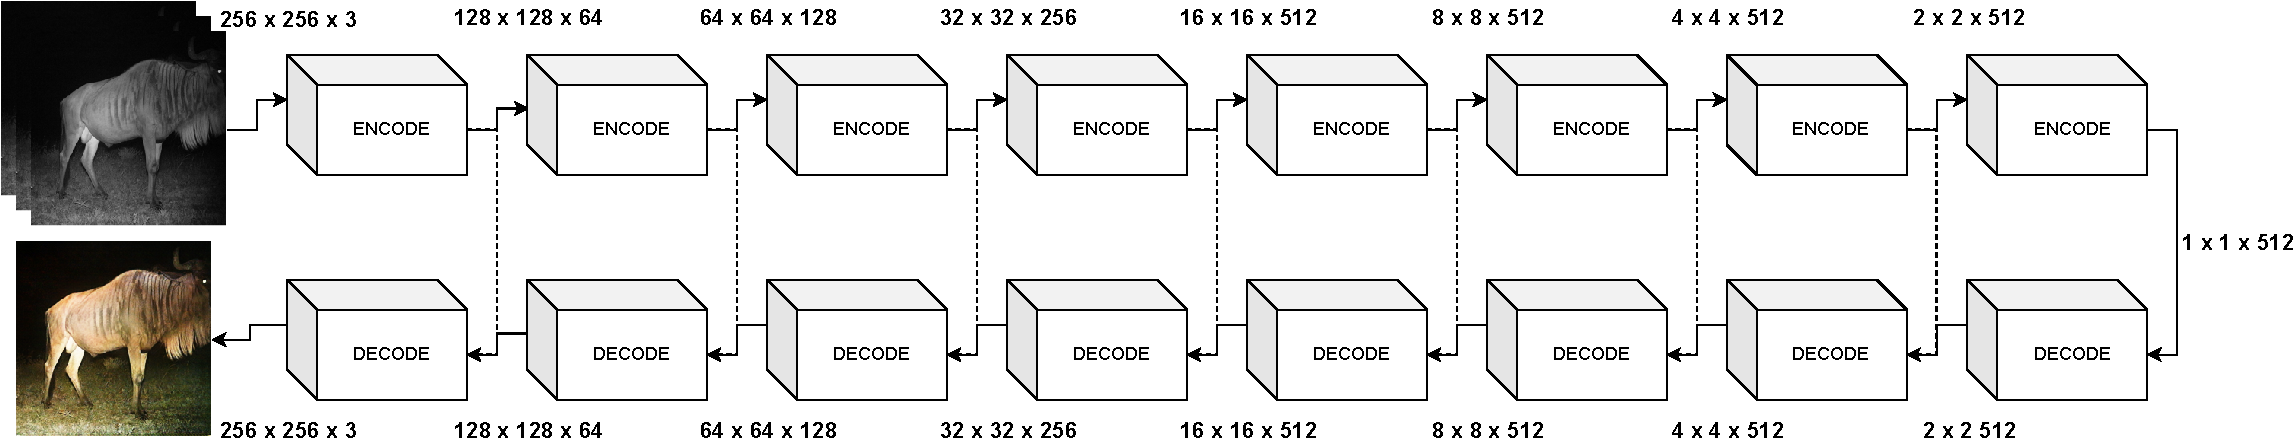
\includegraphics[width=\textwidth]{gfx/CycleGAN-Unet.pdf}
   \caption{U-Net generator $G$ used in CycleGAN \cite{unet,mehri2019colorizing}}
   \label{fig:unet}
\end{figure}

\subsubsection*{Optimizations}
Heusel \textit{et al.} demonstrated that using the \textit{two timescale update rule} (TTUR), which states that when the generator and the discriminator have different learning rates,
mode collapse can be prevented in image translation tasks using GANs \cite{ttur}.
Inspired by this, Mehri \textit{et al.} propose utilizing two learning rates for the CycleGAN architecture \cite{mehri2019colorizing}.

Additionally, Mehri \textit{et al.} propose the use of \textit{spectral normalization}, a technique introduced by Miyato \textit{et al.}, to stabilize the training of the discriminators $D_X$ and $D_Y$ \cite{spectral_norm, mehri2019colorizing}.

Finally, Mehri \textit{et al.} observe that while the cycle consistency loss helps in the early training stages, it hinders the network in the later stages in generating realistic images \cite{mehri2019colorizing}.
Therefore, Mehri \textit{et al.} propose to decrease the weight of the cycle consistency loss after half of the training process \cite{mehri2019colorizing}.

\section{Diffusion Models}
\subsection{Prerequisites}
\subsection{Loss-Based Conditional Sampling}
\subsection{Strong-Guided Conditional Sampling}